\chapter{Robotic arm Python wrapper}
\lhead{\emph{Appendices}} 
\label{app:ros-overview}	
Due to time restriction, the interactions with the physical simulator or the real arms have not been implemented. Despite this, the outline of the physical controller is detailed below for future reference.

\section{Robotic interface}

The Robot Operation System (ROS) provides a software framework to help developers create software involving robots. It includes several open source libraries and tools (BSD license) to "encourage collaborative robotics software development" by providing useful abstraction over hardware, drivers, etc. Since its inception in 2007, ROS has been used to interface with a wide range of robots. Due to the collaborative approach taken by the ROS developers, hundreds of libraries as well as robotic interface have been contributed to the ROS eco-system \cite{noauthor_robot_2017}. This in turn enables developers to concentrate on innovation by building on each other's work. 

ROS is a distributed framework of processes (referred as Nodes in the documentation) performing tasks. The framework is designed to be loosely coupled where each node is supposed to be responsible for a single task. 

The communication between nodes is based on a publish-subscribe pattern using named logical channels called topics. Each node can then send message or receive message by either publishing or subscribing to a topic. ROS also provides services to cope with the need of remote procedure call (RPC) request / reply interactions. The communication protocol is defined by a pair of messages (request and reply). In order for the different node to find each other, ROS provides a Master nodes responsible for the registration as well as the look-up of topics \cite{noauthor_master_nodate}. After successful registration and look-up, the nodes communicate peer-to-peer by publishing a message to a topic or by sending a message to a service. A message is a simple data structure composed of typed fields.

Gazebo provides an open source robot simulation environment. It provides a wide range of tool to help software developers to easily design, test, improve algorithms or robots in realistic scenarios. Gazebo can directly and easily interface with ROS in place of the actual physical robot.

\subsection{Robotic arm}

The physical robotic arm selected was the PhantomX Pincher Robot Mark II \cite{noauthor_phantomx_nodate} or commonly referred as the Turtlebot arm. This arm provides 4 degrees-of-freedom as well as pinching. A model of the arm is available both for ROS and Gazebo. 

\section{Architecture design}

The goal of the physical controller is to abstract and encapsulate the possible action of the different robotic arms.

\subsection{Overview}

\begin{figure}
\centering
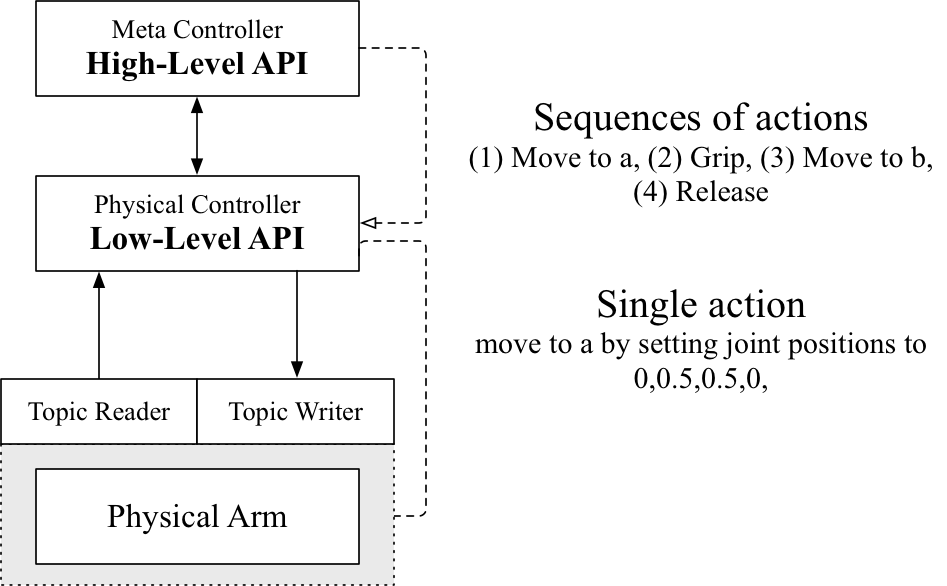
\includegraphics[width=0.7\textwidth]{imgs/ros-gazebo-archi.png}
\caption[Overview of the ROS wrapper architecture]{Overview of the software architecture layers. The greyed items are only here for comprehension purposes and are not part of the physical controller.}
\label{fig:ros-wrapper-architecture}
\end{figure}

Figure ~\ref{fig:ros-wrapper-architecture} shows the different level of abstraction implemented. The interface level provides two abstracted access points to ROS. A topic reader provides access to the latest message published in the topic enable the higher level to know the state of the arm while a topic writer enables the publication of a message to alter the state.

\begin{figure}

\tikzset{
    decision/.style={diamond, draw, fill=blue!20, text width=4.5em, text badly centered, node distance=3cm, inner sep=0pt},
    block/.style={rectangle, draw, fill=blue!20, text width=5em, text centered, rounded corners, minimum height=4em},
    line/.style={draw, -latex'},
    cloud/.style={draw, ellipse,fill=red!20, node distance=3cm, minimum height=2em}
}

\centering
\begin{tikzpicture}[node distance = 2cm, auto]
    % Place nodes
    \node [cloud] (init) {Apply joint position};
    \node [block, below of=init] (apply) {Apply new joint values};
    \node [decision, below= 1cm of apply] (decide1) {reach joint position?};
    \node [decision, below= 1cm of decide1] (decide2) {timeout?};
    \node [cloud, right=1.5cm of decide1] (end) {end};
    \node[left=1.5cm of decide1, scale=0.05](inv){};
    
    % % Draw edges
    \path [line] (init) -- (apply);
    \path [line] (apply) -- node {wait $t$ s} (decide1);
    \path [line] (decide1) -- node {yes}(end);
    \path [line] (decide1) -- node {no}(decide2);
    \path [line] (decide2) -| node[below]{yes}(end);
    
    \path[-,draw] (decide2) -| node[below]{no} (inv.south);
    \path[line]{} (inv.south) |- node{} (apply);
\end{tikzpicture}

\caption[Overview of a controller work-flow]{Example of work-flow abstracted by the arm controller. For the user, after applying a new set of joint position, the controller will either return a zero or non-zero exit status depending on the result of the interaction with the "physical" arm. A non-zero exit code could be returned if a user breaks the arm by applying malicious values.}
\label{fig:ros-controller-process}
\end{figure}


The two interfaces are used to create the physical controller. The goal of the controller is to provide a simple low-level API to interact with the underlying physical object (either real or simulated). The controller abstracts all the steps taken in order to execute an action or raise an exception in case of an error. Figure ~\ref{fig:ros-controller-process} shows the abstracted process for applying new joint angles to the arm. Resting on this process and knowing the joint-position needed to reach point $A$, it is then possible to create a "move to point $A$" endpoints. The architecture leaves the error handling to the user. 

%OpenAI gym framework [REF] is used as a base for the interaction with the environment. It provides a well defined and proved framework for reinforcement learning. Several scenarios have been implemented to enable research with different observation spaces (cameras instead of joint angles, known position of the cube, etc.). It is at the environment level that the exception and failure are currently handled (i.e. reset the arm is case of breakage, etc.).

%\subsection{Limitations}

%Currently the implementation is not capable of the gripping action. Also the robotic arm joints are using the PositionJointInterface [REF] instead of the EffortJointInterface [REF] to simplify the implementation.